\chapter{Схема алгоритма для подсчета МБФ}
Пытаясь улучшить и ускорить алгоритм GEN, мы обнаружили, что одни и те же подфункции
генерериются много раз в разных итерациях главного цикла в GEN.
Их число растет чрезвычайно быстро с ростом числа переменных.
Попытаемся избежать избыточной генерации.
Рассмотрим задачу 
\emph{
"Пусть для фиксированного $n$ в матрице $M_n$ эелемент $m_{i,j} = 0$. 
Сколько МБФ может быть получено с помощью дизъюнкции строки $r_i$ и всех
допустимых строк, у которых индекс $\ge j$".
}
Для решения этой задачи (для $n \leq 7$) мы модифицировали алгоритм GEN, его
новую версию назовем GEN\_Cell. Добавляем в функцию Gen\_I параметр для глубины
рекурсии и счетчик сгенерированных функций (когда глубина равна $0$ возвращаем
значение этого счетчика и запоминаем его, затем сбрасываем счетчик на $0$
для следующего рекурсивного вызова). Полученные числа мы сохраняем в матрице
$Res_n$ размерности $2^n \times 2^n$, элементы которой первоначально равны $0$.
Нам нужно заполнить только те ячейки матрицы $Res_n$, которые соостветствуют 
(т.е. имеют такие же индексы) нулевым элементам, лежащим выше главной диагонали в
$M_n$. Например, для $n=4$ результат представлен 
в таблице 1.
\begin{center}
\label{pic:TableRes_4}
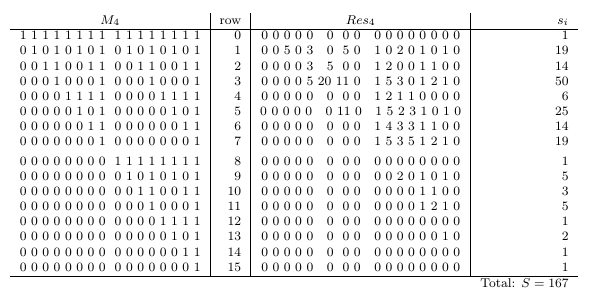
\includegraphics[]{table_res_4_example.png}
\captionof{table}{$M_4,\ Res_4$ и $s_i$ -- число МБФ по строкам}
\end{center}
Легко заметить, что одинаковые подматрицы в $M_4$, более того,
определенное расположение нулей в ней соостветствует такому же расположению
нулей в не нулевых значений в матрице $Res_4$.
Очевидно, что это из-за рекурсивного определения блочной структуры матрицы $M_n$,
характера порождения функций и следовательно характера алгоритма GEN.
Этот факт может быть доказан строго индукцией по $n$ и он демонстрирует свойство
перекрывающих подзадач - одного из ключевых ингридиентов, 
который позволяет нам применить динамическое программирование.
Тоже верно для другого ключевого свойства -- оптимальной подструктуры.
Действительно, если (для фиксированного $n$) подзадача решена, т.е. необходимые 
значения вычислены и сохранены в матрице $Res_n$, то мы можем получить решение
задачи (т.е. найти $\psi(n)$) следующим образом:\par
  (1) находим сумму чисел в $i$-ой строке матрицы $Res_n$ и прибавляем $1$ (т.к.
  каждая строка $M_n$ сама является МБФ). Обозначим эту сумму 
  $s_i,\ i=\overline{0, 2^n - 1}$;\par
  (2) вычисляем $S = \sum\limits_{i=0}^{2^n - 1} s_i$ \par
  (3) полагаем $\psi(n) = S + 1$ (т.к. константу $0$ мы еще не посчитали) и 
  возвращаем его.\par
Например, последний столбец Таблицы 1 содержит суммы $s_i$
элеметов каждого столбца, упомянутые в (1).
Если мы рассмотрим сумму $s_{14} + s_{15} + 1$ (т.к. $M_1$ расположена в нижнем правом
углу $M_4$), то мы получим $3 = \psi(1)$. Если мы сделаем то же самое для 
последних 4-ех строк $s_{12} + \dots + s_{15} + 1$ (т.к. $M_2$ тоже расположена
в нижнем правом углу $M_4$), мы получим $6 = \psi(2)$. 
Для 8-ми последни строк, мы получим $s_8 + \dots + s_{15} + 1 = 20 = \psi(3)$, 
и, наконец, для всех строк мы получим 
$s_0 + \dots + s_{15} + 1 = S + 1 = 168 = \psi(4)$. \par
Следующее улучшение алгоритма GEN\_Cell очевидно: 
после вычисления значений $Res_{n-1}(i, j)$ мы копируем их в соответствующие ячейки, расположенные
аналогично в правом верхнем и нижнем блоке матрицы $Res_n$. Это редотвращает решение одних и тех же 
подзадача более одного раза. Несмотря на это, выполнение GEN\_Cell тольок для одной ячейки может повлечь
генерирование множества подфункций, которые до этого уже генерировались. Их меморизация может занять много времени,
и наша цель -- ограничить генерацию насколько это возможно.
Предположим, что $i < j,\ M_n(i, j) = 0$ и $Res_n(i, j) = 0$. 
Нужно вычислить значение $Res_n(i,j)$, т.е. посчитать все МБФ, которые являются 
дизъюнкциями $i$-й строки $M_n$ со всеми
допустимыми строками $M_n$, индекс которых $\ge j$".
Все элементы $i$-й строки с $j$-го по последний будем рассматривать как вектор
и обозначим его $(0\al)$. Аналогично для $j$-ой строки все элементы с $j$-го по 
последний будем рассматривать как вектор
и обозначим его $(1\be)$.
Для $\al$ и $\be$ имеем 3 случая: (1) $\al \preceq \be;$ (2) $\be \prec \al$, 
и (3) $\al$ и $\be$ несравнимы.
Используя свойства матрицы $M_n$ и доводы, приведенные выше, мы можем доказать:
\begin{Proposition}\label{Prop_alpha_preceq_beta}
 Случай (1): если $\al \preceq \be$, то 
 $Res_n(i,j) = 1 + \sum\limits^{2^n-1}_{k=j+1} Res_n(j,k) = s_j + 1$. 
\end{Proposition}

\begin{Proposition}\label{Prop_beta_prec_alpha}
 Случай (2): если $\be \prec \al$, то 
 $Res_n(i,j) = 1 + \sum\limits^{2^n-1}_{k=j+1} Res_n(i,k)$. 
\end{Proposition}

  Пусть мы уже вычислили $Res_n(i,k)$ и $Res_n(j,k)$ для $k=j+1, \dots, 2^n-1$ и хотим вычислить $Res_n(i,j)$.
Если $\al \preceq \be$ или $\be \prec \al$, то применяем Предложение \ref{Prop_alpha_preceq_beta} или \ref{Prop_beta_prec_alpha} 
соответственно.
Для третьего случая мы используем GEN\_Cell, т.к. мы пока не нашли лучшего алгоритма (или формулы).\par
Следующее предложение следует прямо из определения матрицы $M_n$.

\begin{Proposition}\label{Prop_elements_in_Mn}
Для фиксированного $n$ матрица $M_n$ содержит $4^n$ элементов и:
\newcounter{Prop_elements_in_Mn}
	\begin{list}{\arabic{Prop_elements_in_Mn})}{\usecounter{Prop_elements_in_Mn}} 
	\item $3^n$ из них равны $1$ и они находятся на главной диагонали либо выше неё;
	\item все $(4^n-2^n)/2$ элементов под главной диагональю равны нулю, а также 
	$(4^n - 2\cdot3^n + 2^n)/2$ нулей расположено над главной диагональю.
	\end{list}
\end{Proposition}
Итак, нашему алгоритму нужно вычислить и заполнить $(4^n - 2\cdot3^n + 2^n)/2$ элементов матрицы $Res_n$.
Некоторые из значений получаются в соостветствии с рассмотренными тремя случаями. 
Остальные являются копиями, 
посчитанных значений элементов матрицы $Res_{n-1}$.
Экспериментальные результаты для числа элементов в каждом 
случае для $n=6,7,8$ приведены в Таблице \ref{Table_cases_count_for_Mn}


